\documentclass{article}
\usepackage{graphicx}
\usepackage[margin=1.5cm]{geometry}
\usepackage{amsmath}

\begin{document}
\twocolumn

\title{Warm Up: Energy I}
\author{Prof. Jordan C. Hanson}

\maketitle

\section{Memory Bank}

\begin{itemize}
\item $W = \vec{F} \cdot \Delta \vec{x}$ ... Definition of work
\item $\vec{F} = k\Delta \vec{x}$ ... Hooke's Law, or the force of a spring
\item $W = \frac{1}{2}k(\Delta x)^2$ ... Work done to compress or stretch a spring by $\Delta x$.
\item $KE = \frac{1}{2}m v^2$ ... Definition of Kinetic Energy
\item $W = KE_f - KE_i$ ... Work-energy theorem
\end{itemize}

\section{Work and Energy}

\begin{enumerate}
\item Give an example of something we think of as work that is not work in the scientific sense. Is energy transferred or changed in form in your example? If so, explain how this is accomplished without doing work. \\ \vspace{3cm}
\item In Fig. \ref{fig:work} below, we see a spring that is compressed by $\Delta \vec{x}$.  It turns out that the work done to compress the spring in either direction is $W = \frac{1}{2} k (\Delta x)^2$.  (a) How much work is done to compress a spring with $k = 1000$ N/m a distance of 3 cm, in Joules?  (b) How much work would be done if the distance were tripled?  (c) If the spring were compressed 10 cm and used to launch a mass of 0.1 kg, how much kinetic energy would the object have? \textit{Hint: the kinetic energy is equal to the work done.} (d) How high would the object go? \\ \vspace{5cm}
\end{enumerate}

\begin{figure}
\centering
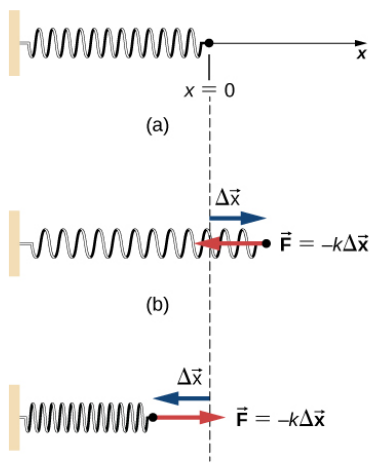
\includegraphics[width=0.33\textwidth]{springWork.png}
\caption{\label{fig:work} When a spring is compressed by a distance $\Delta x$, this requires a force $\vec{F} = k\Delta \vec{x}$ because the spring presses back with $\vec{F} = -k\Delta \vec{x}$.  Compressing the spring requires a \textit{work} $W = \frac{1}{2} k (\Delta x)^2$.}
\end{figure}

\end{document}
